\documentclass{ximera}

\begin{document}
	\author{Stitz-Zeager}
	\xmtitle{TITLE}
\mfpicnumber{1} \opengraphsfile{ExercisesforTheLawofSines} % mfpic settings added 


In Exercises \ref{firstlawofsines} - \ref{lastlawofsines}, solve for the remaining side(s) and angle(s) if possible.  As in the text, $(\alpha, a)$, $(\beta, b)$ and $(\gamma, c)$ are angle-side opposite pairs.

\begin{multicols}{2}

\begin{enumerate}

\item $\alpha = 13^{\circ}, \; \beta = 17^{\circ}, \; a = 5$ \label{firstlawofsines}
\item $\alpha = 73.2^{\circ}, \; \beta = 54.1^{\circ}, \; a = 117$

\setcounter{HW}{\value{enumi}}

\end{enumerate}

\end{multicols}

\begin{multicols}{2} 

\begin{enumerate}

\setcounter{enumi}{\value{HW}}

\item $\alpha = 95^{\circ}, \; \beta = 85^{\circ}, \; a = 33.33$
\item $\alpha = 95^{\circ}, \; \beta = 62^{\circ}, \; a = 33.33$

\setcounter{HW}{\value{enumi}}

\end{enumerate}

\end{multicols}

\begin{multicols}{2} 

\begin{enumerate}

\setcounter{enumi}{\value{HW}}

\item $\alpha = 117^{\circ}, \; a = 35, \; b = 42$
\item $\alpha = 117^{\circ}, \; a = 45, \; b = 42$

\setcounter{HW}{\value{enumi}}

\end{enumerate}

\end{multicols}

\begin{multicols}{2} 

\begin{enumerate}

\setcounter{enumi}{\value{HW}}

\item $\alpha = 68.7^{\circ}, \; a = 88, \; b = 92$
\item $\alpha = 42^{\circ}, \; a = 17, \; b = 23.5$

\setcounter{HW}{\value{enumi}}

\end{enumerate}

\end{multicols}

\begin{multicols}{2} 

\begin{enumerate}

\setcounter{enumi}{\value{HW}}

\item $\alpha = 68.7^{\circ}, \; a = 70, \; b = 90$
\item $\alpha = 30^{\circ}, \; a = 7, \; b = 14$

\setcounter{HW}{\value{enumi}}

\end{enumerate}

\end{multicols}

\begin{multicols}{2} 

\begin{enumerate}

\setcounter{enumi}{\value{HW}}

\item $\alpha = 42^{\circ}, \; a = 39, \; b = 23.5$
\item $\gamma = 53^{\circ}, \; \alpha = 53^{\circ}, \; c = 28.01$ \label{secondarea}

\setcounter{HW}{\value{enumi}}

\end{enumerate}

\end{multicols}

\begin{multicols}{2} 

\begin{enumerate}

\setcounter{enumi}{\value{HW}}

\item $\alpha = 6^{\circ}, \; a = 57, \; b = 100$
\item $\gamma = 74.6^{\circ}, \; c = 3, \; a = 3.05$

\setcounter{HW}{\value{enumi}}

\end{enumerate}

\end{multicols}

\begin{multicols}{2} 

\begin{enumerate}

\setcounter{enumi}{\value{HW}}

\item $\beta = 102^{\circ}, \; b = 16.75, \; c = 13$
\item $\beta = 102^{\circ}, \; b = 16.75, \; c = 18$

\setcounter{HW}{\value{enumi}}

\end{enumerate}

\end{multicols}

\begin{multicols}{2} 

\begin{enumerate}

\setcounter{enumi}{\value{HW}}

\item $\beta = 102^{\circ}, \; \gamma = 35^{\circ}, \; b = 16.75$
\item $\beta = 29.13^{\circ}, \; \gamma = 83.95^{\circ}, \; b = 314.15$

\setcounter{HW}{\value{enumi}}

\end{enumerate}

\end{multicols}

\begin{multicols}{2} 

\begin{enumerate}

\setcounter{enumi}{\value{HW}}

\item $\gamma = 120^{\circ}, \; \beta = 61^{\circ}, \; c = 4$
\item $\alpha = 50^{\circ}, \; a = 25, \; b = 12.5$ \label{lastlawofsines}

\setcounter{HW}{\value{enumi}}

\end{enumerate}

\end{multicols}

\begin{enumerate}

\setcounter{enumi}{\value{HW}}


\item Find the area of the triangles given in Exercises \ref{firstlawofsines}, \ref{secondarea} and \ref{lastlawofsines} above.

\setcounter{HW}{\value{enumi}}

\end{enumerate}

\phantomsection
\label{gradeofroad}
\textbf{The Grade of a Road:} The grade of a road is much like the pitch of a roof (See Example \ref{roofpitchex}) in that it expresses the ratio of rise/run.  In the case of a road, this ratio is always positive because it is measured going uphill and it is usually given as a percentage.  For example, a road which rises 7 feet for every 100 feet of (horizontal) forward progress is said to have a 7\% grade.  However, if we want to apply any Trigonometry to a story problem involving roads going uphill or downhill, we need to view the grade as an angle with respect to the horizontal.  In Exercises \ref{firstroadgrade} - \ref{lastroadgrade}, we first have you change road grades into angles and then use the Law of Sines in an application.

\begin{enumerate}

\setcounter{enumi}{\value{HW}}

\item Using a right triangle with a horizontal leg of length 100 and vertical leg with length 7, show that a 7\% grade means that the road (hypotenuse) makes about a $4^{\circ}$ angle with the horizontal.  (It will not be exactly $4^{\circ}$, but it's pretty close.) \label{firstroadgrade}

\item What grade is given by a $9.65^{\circ}$ angle made by the road and the horizontal?\footnote{I have friends who live in Pacifica, CA and their road is actually this steep.  It's not a nice road to drive.}

\item Along a long, straight stretch of mountain road with a 7\% grade, you see a tall tree standing perfectly plumb alongside the road.\footnote{The word `plumb' here means that the tree is perpendicular to the horizontal.}  From a point 500 feet downhill from the tree, the angle of inclination from the road to the top of the tree is $6^{\circ}$.  Use the Law of Sines to find the height of the tree.  (Hint: First show that the tree makes a $94^{\circ}$ angle with the road.) \label{lastroadgrade}

\setcounter{HW}{\value{enumi}}

\end{enumerate}

Exercises \ref{bearingfirstexercise} - \ref{bearinglastexercise} use the concept of bearings as introduced in Section \ref{bearings}.

\begin{enumerate}

\setcounter{enumi}{\value{HW}}

\item \label{bearingfirstexercise} Find the angle $\theta$ in standard position with $0^{\circ} \leq \theta < 360^{\circ}$ which corresponds to each of the bearings given below.
\enlargethispage{.25in}
\begin{multicols}{4}

\begin{enumerate}

\item due west
\item S$83^{\circ}$E
\item N$5.5^{\circ}$E
\item due south

\setcounter{HWindent}{\value{enumii}}

\end{enumerate}

\end{multicols}

\begin{multicols}{4} 

\begin{enumerate}

\setcounter{enumii}{\value{HWindent}}

\item N$31.25^{\circ}$W
\item S$72^{\circ}41'12''$W\footnote{See Example \ref{degreeex} in Section \ref{AppAngles} for a review of the DMS system.}
\item N$45^{\circ}$E
\item S$45^{\circ}$W

\end{enumerate}

\end{multicols}

\item  The Colonel spots a campfire at a of bearing N$42^{\circ}$E from his current position.  Sarge, who is positioned 3000 feet due east of the Colonel, reckons the bearing to the fire to be N$20^{\circ}$W from his current position.  Determine the distance from the campfire to each man, rounded to the nearest foot.

\item A hiker starts walking due west from Sasquatch Point and gets to the Chupacabra Trailhead before she realizes that she hasn't reset her pedometer.  From the Chupacabra Trailhead she hikes for 5 miles along a bearing of N$53^{\circ}$W which brings her to the Muffin Ridge Observatory.  From there, she knows a bearing of S$65^{\circ}$E will take her straight back to Sasquatch Point.  How far will she have to walk to get from the Muffin Ridge Observatory to Sasquach Point?  What is the distance between Sasquatch Point and the Chupacabra Trailhead?

\item  The captain of the SS Bigfoot sees a signal flare at a bearing of N$15^{\circ}$E from her current location. From his position, the captain of the HMS Sasquatch finds the signal flare to be at a bearing of N$75^{\circ}$W.  If the SS Bigfoot is 5 miles from the HMS Sasquatch and the bearing from the SS Bigfoot to the HMS Sasquatch is N$50^{\circ}$E, find the distances from the flare to each vessel, rounded to the nearest tenth of a mile.

\item  Carl spies a potential Sasquatch nest at a bearing of N$10^{\circ}$E and radios Jeff, who is at a bearing of N$50^{\circ}$E from Carl's position.  From Jeff's position, the nest is at a bearing of S$70^{\circ}$W. If Jeff and Carl are 500 feet apart, how far is Jeff from the Sasquatch nest?  Round your answer to the nearest foot.

\item  A hiker determines the bearing to a lodge from her current position is S$40^{\circ}$W.  She proceeds to hike 2 miles at a bearing of S$20^{\circ}$E at which point she determines the bearing to the lodge is S$75^{\circ}$W.  How far is she from the lodge at this point?  Round your answer to the nearest hundredth of a mile.

\item \label{bearinglastexercise} A watchtower spots a ship off shore at a bearing of N$70^{\circ}$E.  A second tower, which is 50 miles from the first at a bearing of S$80^{\circ}$E from the first tower, determines the bearing to the ship to be N$25^{\circ}$W. How far is the boat from the second tower?  Round your answer to the nearest tenth of a mile.


\setcounter{HW}{\value{enumi}}

\end{enumerate}

\newpage

Exercises \ref{losincliniationdepressionexfirst} -  \ref{losincliniationdepressionexlast} use the concepts of `angle of inclination' and `angle of depression' introduced in Section \ref{AppRightTrig} on page \ref{angleofelevation} and Exercise \ref{angleofdepression}, respectively.


\begin{enumerate}

\setcounter{enumi}{\value{HW}}

\item  \label{losincliniationdepressionexfirst} Skippy and Sally decide to hunt UFOs.  One night, they position themselves 2 miles apart on an abandoned stretch of desert runway.  An hour into their investigation, Skippy spies a UFO hovering over a spot on the runway directly between him and Sally.  He records the angle of inclination from the ground to the craft to be $75^{\circ}$ and radios Sally immediately to find the angle of inclination from her position to the craft is $50^{\circ}$.  How high off the ground is the UFO at this point?  Round your answer to the nearest foot.  (Recall:  1 mile is 5280 feet.)

\item  \label{losincliniationdepressionexlast} The angle of depression from an observer in an apartment complex to a gargoyle on the building next door is $55^{\circ}$.  From a point five stories below the original observer, the angle of inclination to the gargoyle is $20^{\circ}$.  Find the distance from each observer to the gargoyle and the distance from the gargoyle to the apartment complex.  Round your answers to the nearest foot.  (Use the rule of thumb that one story of a building is 9 feet.)  

\setcounter{HW}{\value{enumi}}

\end{enumerate}

\begin{enumerate}
\setcounter{enumi}{\value{HW}}
\item \label{losincliniationdepressionexlast} A villainous trio from a copyrighted anime ascends vertically in their hot air balloon from a point on level ground at a constant rate of $6$ feet per second.  Let $\theta$ be the angle of inclination to the base of the balloon basket from a point on the ground 40 feet away from the launch point.  

\begin{enumerate}

\item Let $h$ denote the height of the balloon off of the ground.  Show $h = 40 \sin(\theta)$.

\item Use the related rate law:\footnote{Theorem \ref{relatedratesaroc} in Section  \ref{RelatedRates}}  $\frac{\Delta h}{\Delta t} = \frac{\Delta h}{\Delta \theta} \, \frac{\Delta \theta}{\Delta t}$ to help you find the rate of change of $\theta$ with respect to time as $\theta$ increases from $60^{\circ}$ to $60.1^{\circ}$.  Remember to give units.

\end{enumerate}


\item  It takes 2 minutes for the 160 foot Ashtabula Bascule Lift Bridge to rotate $45^{\circ}$ from its horizontal position to its raised position, as seen below.\footnote{You can see a video of the bridge being raised  \href{http://www.youtube.com/watch?v=PRwZzzPyK2g}{\underline{here}}.}


\smallskip

\centerline{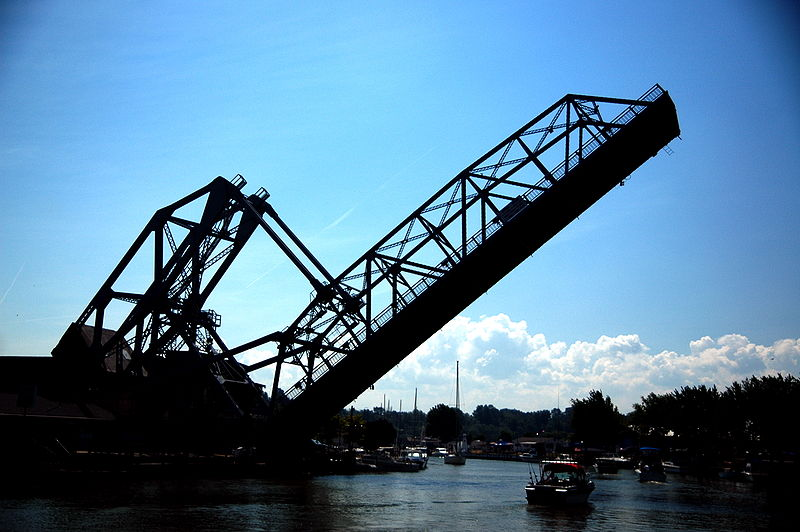
\includegraphics[width=2in]{./LawofSinesGraphics/AshBridge.jpg}}

\smallskip


Assume the bridge casts a shadow directly below itself the entire time it is being raised,\footnote{That is, the sun is directly overhead of the bridge and is shining for an entire two minutes... which never actually happens.} 

\begin{enumerate}

\item  Let $s$ denote the length of the shadow of the bridge on the water.  Show $s = 160 \cos(\theta)$. 
 
\smallskip

\item Assuming  the angle of elevation of the bridge changes at a constant rate, use the related rate law:\footnote{Theorem \ref{relatedratesaroc} in Section  \ref{RelatedRates}} $\frac{\Delta s}{\Delta t} = \frac{\Delta s}{\Delta \theta} \, \frac{\Delta \theta}{\Delta t}$   to help you find the rate of change of the shadow length with respect to time as $\theta$ increases from $30^{\circ}$ to $30.1^{\circ}$.  Remember to give units.


\end{enumerate}

\setcounter{HW}{\value{enumi}}
\end{enumerate}

\begin{enumerate}
\setcounter{enumi}{\value{HW}}

\item Prove that the Law of Sines holds when $\triangle ABC$ is a right triangle.

\item Discuss with your classmates why knowing only the three angles of a triangle is not enough to determine any of the sides.

\item Discuss with your classmates why the Law of Sines cannot be used to find the angles in the triangle when only the three sides are given.  Also discuss what happens if only two sides and the angle between them are given.  (Said another way, explain why the Law of Sines cannot be used in the SSS and SAS cases.)

\item Given $\alpha = 30^{\circ}$ and $b = 10$, choose four different values for $a$ so that 

\begin{enumerate}

\item the information yields no triangle
\item the information yields exactly one right triangle
\item the information yields two distinct triangles
\item the information yields exactly one obtuse triangle

\end{enumerate}

Explain why you cannot choose $a$ in such a way as to have $\alpha = 30^{\circ}$, $b = 10$ and your choice of $a$ yield only one triangle where that unique triangle has three acute angles.

\item Use the cases and diagrams in the proof of the Law of Sines (Theorem \ref{lawofsines}) to prove the area formulas given in Theorem \ref{areaformulasine}.  Why do those formulas yield square units when four quantities are being multiplied together?

\setcounter{HW}{\value{enumi}}

\end{enumerate}

\newpage

\subsection{Answers}

\begin{multicols}{2}

\begin{enumerate}

\item $\begin{array}{lll}
\alpha = 13^{\circ} & \beta = 17^{\circ} & \gamma = 150^{\circ} \\
a = 5 & b \approx 6.50 & c \approx 11.11 \end{array}$

\item $\begin{array}{lll}
\alpha = 73.2^{\circ} & \beta = 54.1^{\circ} & \gamma = 52.7^{\circ} \\
a = 117 & b \approx 99.00 & c \approx 97.22 \end{array}$

\setcounter{HW}{\value{enumi}}

\end{enumerate}

\end{multicols}

\begin{multicols}{2} 

\begin{enumerate}

\setcounter{enumi}{\value{HW}}

\item \begin{tabular}{l}
Information does not \\
produce a triangle \end{tabular}

\item $\begin{array}{lll}
\alpha = 95^{\circ} & \beta = 62^{\circ} & \gamma = 23^{\circ} \\
a = 33.33 & b \approx 29.54 & c \approx 13.07 \end{array}$

\setcounter{HW}{\value{enumi}}

\end{enumerate}

\end{multicols}

\begin{multicols}{2} 

\begin{enumerate}

\setcounter{enumi}{\value{HW}}

\item \begin{tabular}{l}
Information does not \\
produce a triangle \end{tabular}

\item $\begin{array}{lll}
\alpha = 117^{\circ} & \beta \approx 56.3^{\circ} & \gamma \approx 6.7^{\circ} \\
a = 45 & b = 42 & c \approx 5.89 \end{array}$

\setcounter{HW}{\value{enumi}}

\end{enumerate}

\end{multicols}

\begin{multicols}{2} 

\begin{enumerate}

\setcounter{enumi}{\value{HW}}

\item $\begin{array}{lll}
\alpha = 68.7^{\circ} & \beta \approx 76.9^{\circ} & \gamma \approx 34.4^{\circ} \\
a = 88 & b = 92 & c \approx 53.36 \end{array}$

$\begin{array}{lll}
\alpha = 68.7^{\circ} & \beta \approx 103.1^{\circ} & \gamma \approx 8.2^{\circ} \\
a = 88 & b = 92 & c \approx 13.47\end{array}$

\item $\begin{array}{lll}
\alpha = 42^{\circ} & \beta \approx 67.66^{\circ} & \gamma \approx 70.34^{\circ} \\
a = 17 & b = 23.5 & c \approx 23.93 \end{array}$

$\begin{array}{lll}
\alpha = 42^{\circ} & \beta \approx 112.34^{\circ} & \gamma \approx 25.66^{\circ} \\
a = 17 & b = 23.5 & c \approx 11.00 \end{array}$

\setcounter{HW}{\value{enumi}}

\end{enumerate}

\end{multicols}

\begin{multicols}{2} 

\begin{enumerate}

\setcounter{enumi}{\value{HW}}

\item \begin{tabular}{l}
Information does not \\
produce a triangle \end{tabular}

\item $\begin{array}{lll}
\alpha = 30^{\circ} & \beta = 90^{\circ} & \gamma = 60^{\circ} \\
a = 7 & b = 14 & c = 7\sqrt{3} \end{array}$

\setcounter{HW}{\value{enumi}}

\end{enumerate}

\end{multicols}

\begin{multicols}{2} 

\begin{enumerate}

\setcounter{enumi}{\value{HW}}

\item $\begin{array}{lll}
\alpha = 42^{\circ} & \beta \approx 23.78^{\circ} & \gamma \approx 114.22^{\circ} \\
a = 39 & b = 23.5 & c \approx 53.15 \end{array}$

\item $\begin{array}{lll}
\alpha = 53^{\circ} & \beta = 74^{\circ} & \gamma = 53^{\circ} \\
a = 28.01 & b \approx 33.71 & c = 28.01 \end{array}$

\setcounter{HW}{\value{enumi}}

\end{enumerate}

\end{multicols}

\begin{multicols}{2} 

\begin{enumerate}

\setcounter{enumi}{\value{HW}}

\item $\begin{array}{lll}
\alpha = 6^{\circ} & \beta \approx 169.43^{\circ} & \gamma \approx 4.57^{\circ} \\
a = 57 & b = 100 & c \approx 43.45 \end{array}$

$\begin{array}{lll}
\alpha = 6^{\circ} & \beta \approx 10.57^{\circ} & \gamma \approx 163.43^{\circ} \\
a = 57 & b = 100 & c \approx 155.51 \end{array}$

\item $\begin{array}{lll}
\alpha \approx 78.59^{\circ} & \beta \approx 26.81^{\circ} & \gamma = 74.6^{\circ} \\
a = 3.05 & b \approx 1.40 & c = 3 \end{array}$

$\begin{array}{lll}
\alpha \approx 101.41^{\circ} & \beta \approx 3.99^{\circ} & \gamma = 74.6^{\circ} \\
a = 3.05 & b \approx 0.217 & c = 3 \end{array}$

\setcounter{HW}{\value{enumi}}

\end{enumerate}

\end{multicols}

\begin{multicols}{2} 

\begin{enumerate}

\setcounter{enumi}{\value{HW}}

\item $\begin{array}{lll}
\alpha \approx 28.61^{\circ} & \beta = 102^{\circ} & \gamma \approx 49.39^{\circ} \\
a \approx 8.20 & b = 16.75 & c = 13 \end{array}$

\item \begin{tabular}{l}
Information does not \\
produce a triangle \end{tabular}

\setcounter{HW}{\value{enumi}}

\end{enumerate}

\end{multicols}

\begin{multicols}{2} 

\begin{enumerate}

\setcounter{enumi}{\value{HW}}

\item $\begin{array}{lll}
\alpha = 43^{\circ} & \beta = 102^{\circ} & \gamma = 35^{\circ} \\
a \approx 11.68 & b = 16.75 & c \approx 9.82 \end{array}$

\item $\begin{array}{lll}
\alpha = 66.92^{\circ} & \beta = 29.13^{\circ} & \gamma = 83.95^{\circ} \\
a \approx 593.69 & b = 314.15 & c \approx 641.75 \end{array}$

\setcounter{HW}{\value{enumi}}

\end{enumerate}

\end{multicols}

\begin{multicols}{2} 

\begin{enumerate}

\setcounter{enumi}{\value{HW}}

\item \begin{tabular}{l}
Information does not \\
produce a triangle \end{tabular}

\item $\begin{array}{lll}
\alpha = 50^{\circ} & \beta \approx 22.52^{\circ} & \gamma \approx 107.48^{\circ} \\
a = 25 & b = 12.5 & c \approx 31.13 \end{array}$

\setcounter{HW}{\value{enumi}}

\end{enumerate}

\end{multicols}

\begin{enumerate}

\setcounter{enumi}{\value{HW}}

\item The area of the triangle from Exercise \ref{firstlawofsines} is about 8.1 square units.\\
The area of the triangle from Exercise \ref{secondarea} is about 377.1 square units.\\
The area of the triangle from Exercise \ref{lastlawofsines} is about 149 square units.

\item $\arctan\left(\frac{7}{100}\right) \approx 0.699$ radians, which is equivalent to $4.004^{\circ}$
\item About 17\%
\item About 53 feet

\pagebreak

\item \begin{multicols}{4} \begin{enumerate}

\item $\theta = 180^{\circ}$
\item $\theta = 353^{\circ}$
\item $\theta = 84.5^{\circ}$
\item $\theta = 270^{\circ}$

\setcounter{HWindent}{\value{enumii}}

\end{enumerate}

\end{multicols}

\begin{multicols}{4} 

\begin{enumerate}

\setcounter{enumii}{\value{HWindent}}

\item $\theta = 121.25^{\circ}$
\item $\theta = 197^{\circ} 18' 48''$
\item $\theta = 45^{\circ}$
\item $\theta = 225^{\circ}$

\end{enumerate}

\end{multicols}

\item  The Colonel is about 3193 feet from the campfire. \\
Sarge is about 2525 feet to the campfire.

\item The distance from the Muffin Ridge Observatory to Sasquach Point is about 7.12 miles.\\
The distance from Sasquatch Point to the Chupacabra Trailhead is about 2.46 miles.

\item  The SS Bigfoot is about 4.1 miles from the flare. \\
The HMS Sasquatch is about 2.9 miles from the flare.

\item  Jeff is about 371 feet from the nest.

\item  She is about 3.02 miles from the lodge

\item  The boat is about 25.1 miles from the second tower.

\item  The UFO is hovering about 9539 feet above the ground.

\item The gargoyle is about 44 feet from the observer on the upper floor. \\
The gargoyle is about 27 feet from the observer on the lower floor. \\
The gargoyle is about 25 feet from the other building.

\setcounter{HW}{\value{enumi}}
\end{enumerate}

\begin{enumerate}
\setcounter{enumi}{\value{HW}}
\item \begin{enumerate} \addtocounter{enumii}{1}

\item  $\frac{\Delta h}{\Delta t}$ is given as a constant $6 \, \frac{\text{ft}}{\text{s}}$. $\frac{\Delta h}{\Delta \theta} = \frac{h(60.1) - h(60)}{0.1} \approx 0.348 \, \frac{\text{ft}}{\text{degree,  } \,  \circ}$.  

\smallskip

Hence, $\frac{\Delta \theta}{\Delta t} = \frac{ 6 \, \frac{\text{ft}}{\text{s}}   }{ 0.348 \, \frac{\text{ft}}{\text{degree,  } \, \circ}} \approx 17.215 \, \frac{ \text{degree,  } \, \circ}{s}$.  

\smallskip

The angle of elevation is increasing at an average rate of $17.215$ degrees  per second.  

\smallskip

\textbf{WARNING:} For (good) reasons you'll explore more deeply in Calculus, you'll usually stick with radians when the Calculus version of this problem rolls around \ldots  

\end{enumerate}


\item  \begin{enumerate} \addtocounter{enumii}{1}

\item   $\frac{\Delta s}{\Delta \theta} = \frac{s(30.1) - s(30)}{0.1} \approx -1.398 \, \frac{\text{ft}}{\text{degree} \,  \circ}$.  

\smallskip

We are told to assume $\frac{\Delta \theta }{\Delta t}$ is a constant, so $\frac{\Delta s}{\Delta t} = \frac{45^{\circ}}{2 \, \text{minutes}} = 22.5 \, \frac{\text{degree,  } \, \circ}{\text{min}}$.

\smallskip

We get:  $\frac{\Delta s}{\Delta t} = \frac{\Delta s}{\Delta \theta} \, \frac{\Delta \theta }{\Delta t} \approx \left(-1.398 \, \frac{\text{ft}}{\text{degree,  } \,  \circ} \right) \left(  22.5 \, \frac{\text{degree,  } \, \circ}{\text{min}} \right) \approx -31.436 \, \frac{\text{ft}}{\text{min}}$.

\smallskip

This means the shadow is receding at a rate of approximately 31.436 feet per minute.

\smallskip

\textbf{WARNING:} For (good) reasons you'll explore more deeply in Calculus, you'll usually stick with radians when the Calculus version of this problem rolls around \ldots  

\end{enumerate}


\setcounter{HW}{\value{enumi}}
\end{enumerate}




\end{document}
